\chapter{Verification and Validation Process}

\section{Verification Methods}

Verification methods are all methods to proof a implementation adheres to its given requirements. 

\subsection{Analysis}
\subsection{Inspection}

An inspection is done in groups not smaller then two people, where at least one person who has not contributed to the unit under inspection is present.

An inspection's purpose is to verify the correct implementation of a given requirement, which can not be tested using automated tests, as per chapter \ref{sec:Test}.

\subsection{Test}
\label{sec:Test}

A test verifying a requirement must be implemented by a person, who has not contributed to the unit under test. This rule may be relaxed for integration tests, where multiple people have contributed to the system under test. In that case no test shall be executed without verification by inspection by at least on other person.

A test of VHDL code shall be performed using Vivado's builtin simulation suite. A test shall use assert statements to automatically falsify an executed test, if the tested requirement is not fullfilled.

\section{Validation Methods}
\subsection{Inspection}
\subsection{Demonstration}

A demonstration is conducted either using a simulation or using an implementation of the developed system under test, which is loaded into the target FPGA. It does not specifically verify any requirement, but serves to show a customer the correct high level functionality requested.

\subsection{Test}

\chapter{Verification and Validation Implementation}

\chapter{End Item Verification and Validation}
% White Box Verification
The white box tests are designed to demonstrate the compliance with the CCSDS' requirements and aid in the continuous integration of the product. 


\section{CCSDS 132 Encoder}


\section{CCSDS 131 Encoder / Decoder}

The development of the CCSDS 131 Encoder and Decoder end items is closely coupled. Therefore, all verfication and validation activities are done together for both subsystems. This not only simplifies planning but also allows the employment of better verification methods.

\subsection{Engineering Unit Evaluations}

No strict guidelines are given for the development of the end items. As per the set development process every developed unit shall have appropriate unit tests to verify correct functionality.

\subsection{Verification Activities}

The verification activities aim to cover 100 \% of the system's low level requirements, either by defining test cases to be tested in a testing campaign or, where tests are not applicable / possible, by inspection in a code walkthrough.


\subsubsection{Verification by Testing}

\paragraph{GND-REQ-3}
\paragraph{GND-REQ-4}
\paragraph{GND-REQ-15}
\paragraph{GND-REQ-16}
\paragraph{SPC-REQ-2}
\paragraph{SPC-REQ-3}
\paragraph{SPC-REQ-13}
\paragraph{SPC-REQ-16}
\paragraph{SPC-REQ-17}
\paragraph{SYS-REQ-1}
\paragraph{SYS-REQ-2}


\subsubsection{Verification by Inspection}

\paragraph{Inspection RNG and ASM} Git Hash 6816daf: 01.06.2026
\begin{table}[h!]
	\begin{tabular}{|c|c|c|c|}
		\hline
		\textbf{Covered Requirement} & \textbf{Imp. Developer} & \textbf{Ver. Developer} & \textbf{PASS/FAIL}\\
		\hline
		GND-REQ-11 & HL & MF LR & PASS \\
		\hline
		GND-REQ-13 & HL & MF LR & PASS \\
		\hline
		SPC-REQ-23 & HL & MF LR & PASS \\
		\hline
		SPC-REQ-24 & HL & MF LR & PASS \\
		\hline
		SYS-REQ-3 & HL & MF LR & PASS \\
		\hline
		SYS-REQ-4 & HL & MF LR & PASS \\
		\hline
		NFUNC-REQ-1 & HL & MF LR & FAIL, AXI Signale \\
		\hline
		NFUNC-REQ-2 & HL & MF LR & PASS \\
		\hline
		SPC-REQ-26 & HL & MF LR & PASS \\
		\hline
	\end{tabular}
	\caption{Requirements covered by Inspection RNG and ASM.}
	\label{tab:inspec_RNG_ASM}
\end{table}


\paragraph{Inspection Reed Solomon} Git Hash 7ed3168: 01.06.2026

\begin{table}[H]
	\begin{tabular}{|c|c|c|c|}
		\hline
		\textbf{Covered Requirement} & \textbf{Imp. Developer} & \textbf{Ver. Developer} & \textbf{PASS/FAIL}\\
		\hline
		GND-REQ-1 & MF & HL LR & PASS \\
		\hline
		GND-REQ-12 &MF & HL LR & PASS \\
		\hline
		GND-REQ-15 &MF & HL LR & PASS\\
		\hline
		GND-REQ-16 &MF & HL LR & PASS\\
		\hline
		SPS-REQ-22 &MF & HL LR& PASS \\
		\hline
		SYS-REQ-5 &MF & HL LR& PASS\\
		\hline
		SYS-REQ-6 &MF & HL LR& PASS\\
		\hline
		SYS-REQ-9 &MF & HL LR& PASS\\
		\hline
		NFUNC-REQ-1 &MF & HL LR& FAIL\\
		\hline
		NFUNC-REQ-2 & MF & HL LR& FAIL\\
		\hline
		SPC-REQ-26 & MF & HL LR & FAIL\\
		\hline
	\end{tabular}
	\caption{Requirements covered by Reed Solomon}
	\label{tab:inspec_R_S}
\end{table}


\paragraph{Inspection Convolutional Code} Git Hash 6816daf: 01.06.2026
\begin{table}[H]
	\begin{tabular}{|c|c|c|c|}
		\hline
		\textbf{Covered Requirement} & \textbf{Imp. Developer} & \textbf{Ver. Developer} & \textbf{PASS/FAIL}\\
		\hline
		GND-REQ-2 & LR & MF HL & PASS \\
		\hline
		GND-REQ-4 & LR & MF HL & PASS \\
		\hline
		GND-REQ-6 & LR & MF HL & PASS \\
		\hline
		SPS-REQ-5 & LR & MF HL & PASS \\
		\hline
		SPS-REQ-21 & LR MF & HL & PASS \\
		\hline
		SPS-REQ-25 & LR & MF HL & PASS \\
		\hline
		SYS-REQ-7 & LR & MF HL & PASS \\
		\hline
		SYS-REQ-8 & LR & MF HL & PASS \\
		\hline
		NFUNC-REQ-1 & LR & MF HL & FAIL, AXI Signale, Reset \\
		\hline
		NFUNC-REQ-2 & LR & MF HL & PASS \\
		\hline
		SPC-REQ-26 & LR & MF HL & PASS \\
		\hline
	\end{tabular}
	\caption{Requirements covered by Convolutional Code}
	\label{tab:inspec_C_C}
\end{table}


\subsubsection{Verification by Analysis}

\paragraph{GND-REQ-14}
\paragraph{SPC-REQ-1}
\paragraph{SPC-REQ-2}
\paragraph{SPC-REQ-4}
\paragraph{SPC-REQ-6}
\paragraph{SPC-REQ-8}

\section{Validation Activities}

\subsection{Verification by Testing}

\section{CCSDS 131 Decoder}
\section{CCSDS 132 Decoder}


\chapter{System Verification and Validation}
% Black Box End to End Validation
The purpose of the black box test is not to verify the correct implementation of the CCSDS' requirements, but rather to validate that no data is lost and the desired data rate is achievable. 

This requires the entire processing chain to be fully integrated, with a system in place to simulate the On-Board Computer (OBC), which handles data generation and comparison of the generated data with the output of the integrated chain. This Testsystem will be run on the target hardware to also demonstrate the correct synthesis and implementation of the devloped product. The described architecture is visualized in Figure \ref{fig:testsystem}

\begin{figure}
	\centering
	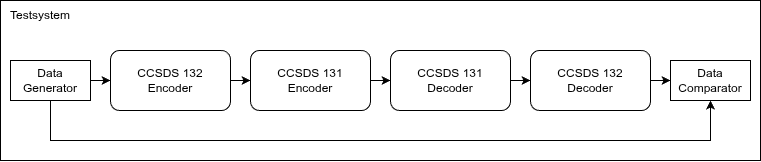
\includegraphics[width=\linewidth]{img/TestSystemSketch.drawio.png}
	\caption{End to End Testsystem}
	\label{fig:testsystem}
\end{figure}

\section{Test A}
\subsection{Test Definition}
\subsection{Test Result}

\section{Test B}
\subsection{Test Definition}
\subsection{Test Result}
